\documentclass[usenames,dvipsnames,10pt,aspectratio=169]{beamer}
\usepackage[absolute,overlay]{textpos}
%\usefonttheme{professionalfonts}

% Setup appearance:
\usetheme{Boadilla}
\usefonttheme[onlylarge]{structurebold}
\usecolortheme{seahorse}
\setbeamerfont*{frametitle}{size=\normalsize,series=\bfseries}
\setbeamerfont{frametitle}{size=\large}
\setbeamertemplate{navigation symbols}{}
%\setbeamercolor{frametitle}{fg=Blue}
\renewcommand\alert[1]{{\color{Magenta} #1}}
\newcommand\program[1]{\texttt{#1}}

% Packages
\usepackage[english,ukrainian]{babel}
\usepackage[T1]{fontenc}
\usepackage{lmodern}
\usepackage[utf8]{inputenc}
\usepackage{color}
\usepackage{bm}
\usepackage{slashed}
\usepackage{booktabs}% http://ctan.org/pkg/booktabs
\usepackage{xspace}
\usepackage{multirow}
\usepackage{graphicx}
\newcommand{\tabitem}{~~\llap{\textbullet}~~}
\usepackage{minted}
\usepackage{scalerel}

\setlength{\fboxsep}{0pt}%
\setlength{\fboxrule}{1pt}%

%\definecolor{stcoupcolor}{RGB}{255,0,51}

% Setup TikZ
\usepackage{tikz}
\usetikzlibrary{arrows,shapes,backgrounds,positioning}
\tikzstyle{block}=[draw opacity=0.7,line width=1.4cm]

% arrows
\tikzset{
	myarrow/.style={
		draw,
		fill=orange,
		single arrow,
		rounded corners=1,
		%        width=2ex,
		minimum width=2ex,
		minimum height=3ex,
		single arrow head extend=1ex
	}
}
\newcommand{\arrowup}{\tikz [baseline=-0.5ex]{\node [myarrow,rotate=90] {};}}
\newcommand{\arrowdown}{\tikz [baseline=-0.5ex]{\node [myarrow,rotate=-90] {};}}
\newcommand{\arrowright}{\tikz [baseline=-0.5ex]{\node [myarrow,rotate=0] {};}}
\newcommand{\arrowleft}{\tikz [baseline=-0.5ex]{\node [myarrow,rotate=180] {};}}

% draw connection
\newcommand{\tikzmark}[1]{\tikz[remember picture] \node[coordinate] (#1) {#1};}

% page numbering (backup)
\newcommand{\backupbegin}{\newcounter{finalframe}\setcounter{finalframe}{\value{framenumber}}}
\newcommand{\backupend}{\setcounter{framenumber}{\value{finalframe}}}

% Author, Title, etc.
\title[ROOT. Реконструкція інваріантної маси]{\large Знайомство з ROOT:\newline реконструкція інваріантної маси частинок}
\author[Олександр Зенаєв]{Олександр Зенаєв}
\date{}

% block with custom width
\newenvironment<>{varblock}[2][.9\textwidth]{%
    \setlength{\textwidth}{#1}
    \begin{actionenv}#3%
        \def\insertblocktitle{#2}%
        \par%
        \usebeamertemplate{block begin}}
    {\par%
        \usebeamertemplate{block end}%
\end{actionenv}}

\setbeamertemplate{itemize/enumerate body begin}{\footnotesize}
\setbeamertemplate{itemize/enumerate subbody begin}{\footnotesize}

\tikzset{
    every overlay node/.style={
        rounded corners,anchor=north west,
    },
}
\def\tikzoverlay{%
    \tikz[baseline,overlay]\node[every overlay node]
}%

% main part
\begin{document}
    \begin{frame}[plain]
    %\centering\includegraphics[width=0.15\textwidth]{pics/logo/cms.png}
    %\hspace{0.1\textwidth}
    %\centering\includegraphics[width=0.18\textwidth]{pics/logo/h1}
    %\hspace{0.1\textwidth}
    %\centering\includegraphics[width=0.15\textwidth]{pics/logo/desyNEW}
    %\hspace{0.1\textwidth}
    %\centering\includegraphics[width=0.15\textwidth]{pics/logo/zeus}
    %\hspace{0.1\textwidth}
    %\centering\includegraphics[width=0.15\textwidth]{pics/logo/xFitterLogo1.png}
    
    \vspace{-0.05\textheight}
    \titlepage
    
    %\vspace{-0.15\textheight}
    %\centering\includegraphics[width=0.4\textwidth]{pics/titlepic.jpg}

    %\vspace{-0.15\textheight}
    %{\color{blue} Overview:}
    
    \vspace{0.04\textheight}
    \centering
    %place \\
    %date
\end{frame}

% number of slides w/out backup
\renewcommand{\inserttotalframenumber}{2}
\setbeamercolor{footline}{fg=blue}
\setbeamerfont{footline}{series=\bfseries}


\begin{frame}
\frametitle{ROOT $~~~~~$ \url{https://root.cern/}}
\begin{minipage}{0.685\textwidth}
ROOT -- це програмний пакет для зберігання, аналізу та візуалізації великих обсягів даних, який широко використовується у фізиці високих енергій

\begin{itemize}
	\item відкрите програмне забезпечення (фреймворк), розробляється у CERN (Європейській організації з ядерних досліджень) 1995--\dots
	\item написаний на С++, має інтерактивний інтерпретатор, підтримує інтеграцію з іншими мовами, такими як Python (через інтерфейс PyROOT)
	\item основне застосування:
	\begin{itemize}
		\item зберігання та зчитування великих обсягів даних
		\item статистичний аналіз даних
		\item візуалізація
	\end{itemize}
	\item підтримує паралельні обчислення
	\item має широку підтримку наукової спільноти (документація, приклади, форум \url{https://root-forum.cern.ch/})
\end{itemize}
\end{minipage}
\begin{minipage}{0.05\textwidth}
\end{minipage}
\begin{minipage}{0.295\textwidth}
\centering{
\includegraphics[width=1.0\textwidth]{pics/logo_full-plus-text-ver.png}}
\end{minipage}

%\begin{columns}\column{\dimexpr\paperwidth-10pt}
%\centering{\includegraphics[width=1.0\textwidth]{pics/pic.png}}
%\end{columns}
\end{frame}

\begin{frame}[fragile]
	\frametitle{Початок роботи з ROOT: інтерпретатор, компіляція}

\begin{tabular}{|p{0.43\textwidth}|p{0.51\textwidth}|}
	\hline
	ROOT інтерпретатор & C++ компілятор із ROOT бібліотекою \\
	\hline
	{\scriptsize
\begin{minted}{c++}
// hello.cpp
	
void hello() {
	printf("Hello world\n");
	TH1F hist("hist", "My histo", 300, 0., 3.);
	hist.Fill(1.2);
	hist.Print();
}
\end{minted}
	} & 
	{\scriptsize
		\begin{minted}{c++}
// hello_main.cpp

#include <cstdio>
#include <TH1F.h>
int main() {
	printf("Hello world\n");
	TH1F hist("hist", "My histo", 300, 0., 3.);
	hist.Fill(1.2);
	hist.Print();
	return 0;
}
		\end{minted} 
	}
	\\ \hline
	{ \scriptsize
	\begin{minted}{bash}
root -l -q hello.cpp		
	\end{minted} 
	} &
	{ \scriptsize
	\begin{minted}{bash}
g++ -o hello_main `root-config --cflags --libs` hello_main.cpp
./hello_main
\end{minted}
	}
	\\ \hline
{ \scriptsize
	\begin{minted}{bash}

Processing hello.cxx...
Hello world
TH1.Print Name  = hist, Entries= 1, Total sum= 1
	\end{minted} 
} &
{ \scriptsize
	\begin{minted}{bash}
Hello world
TH1.Print Name  = hist, Entries= 1, Total sum= 1
	\end{minted}
}
\\ \hline
\end{tabular}

\end{frame}

\begin{frame}[fragile]
	\frametitle{Початок роботи з ROOT: PyROOT}
	\begin{itemize}
		\item PyROOT: Python інтерфейс до ROOT
		\begin{itemize}
			\item дуже зручний для прототипування (дослідницький код)
			\item багато корисних Python модулів (numpy, pandas, matplotlib \dots) + документація і дуже велика спільнота
		\end{itemize}
	\end{itemize}
\rule{\textwidth}{1pt}
{ \scriptsize
	\begin{minted}{python}
# hello.py

import ROOT

if __name__ == '__main__':
  print("Hello world")
  hist = ROOT.TH1F("hist", "My histo", 300, 0., 3.)
  hist.Fill(1.2)
  hist.Print()
	\end{minted} 
}
\rule{\textwidth}{1pt}
{ \scriptsize
	\begin{minted}{bash}
python hello.py
	\end{minted} 
}
\rule{\textwidth}{1pt}
{ \scriptsize
	\begin{minted}{bash}
Hello world
TH1.Print Name  = hist, Entries= 1, Total sum= 1
	\end{minted} 
}
\rule{\textwidth}{1pt}

\end{frame}

\begin{frame}
	\frametitle{Реконструкція інваріантної \newline маси (системи) частинок}
	\begin{minipage}{0.4\textwidth}
	\begin{itemize}
	\item Реконструкція інваріантної маси -- важлива складова аналізу даних експериментів у HEP
	\begin{itemize}
		\item дослідження властивостей частинок (вимірювання маси, ширини розпаду тощо)
		\item вимірювання перерізів народження частинок
	\end{itemize}
	\end{itemize}
	\end{minipage}
	\begin{minipage}{0.59\textwidth}

	\vspace{-0.18\textheight}
	\hspace*{0.0\textwidth}{\vstretch{.78}{\includegraphics[width=1.1\textwidth]{pics/cms.png}}}
	\end{minipage}
		
	\vspace{0.025\textheight}
	\begin{itemize}
		\item Інваріантна маса
		$M = E^2-P^2 = (E_1+E_2)^2-(P_1+P_2)^2$ 
		не змінюється при перетворенні системи відліку
		\item Експериментальні дані складаються з числених \underline{подій} (одне зіткнення частинок)
		\item Дані про кожну \underline{подію} містять енергії та/чи імпульси зареєстрованих детектором (стабільних чи довгоживучих) частинок
		\begin{itemize}
			\item трекова система в магнітному полі рекенструює \underline{треки} (tracks) (імпульси для заряджених частинок)
			%\item система ідентифікації частинок (Черенковський детектор, або за втратами енергії $dE/dx$) дозволяє ідентифікувати тип частинки (Particle Identification, PID) $\to$ дізнатися її масу (піон/каон) $\to$ енергію
			\item система ідентифікації частинок (Particle Identification, PID)cвизначає тип частинки (маса)
			\item[] $\to$ це дозволяє \emph{реконструювати} (тобто обчислити енергію та імпульс) батьківської нестабільної частинки, яку хочемо досліджувати і яка не може бути зареєстрована детектором
		\end{itemize}
		\item Аналіз даних потребує фільтрацію шуму, корекцію детекторних ефектів тощо
		\begin{itemize}
			\item зазвичай народжується багато нестабільних частинок $\to$ десятки, сотні чи навіть тисячі треків у кожній події $\to$ тисячі чи мільони \underline{комбінацій} (комбінаторний фон)
		\end{itemize}
	\end{itemize}
\end{frame}

\begin{frame}
	\frametitle{Реконструкція інваріантної маси $D^{+}\to K^{-}\pi^{+}\pi^{+}$ }
	
	{\scriptsize ZEUS Coll., H. Abramowicz et al., ``Measurement of $D^{\pm}$ production in deep
		inelastic $ep$ scattering with the ZEUS detector at HERA'', JHEP05 (2013) 023 \href{https://arxiv.org/abs/1302.5058}{[arXiv:1302.5058]}}
	
	\centering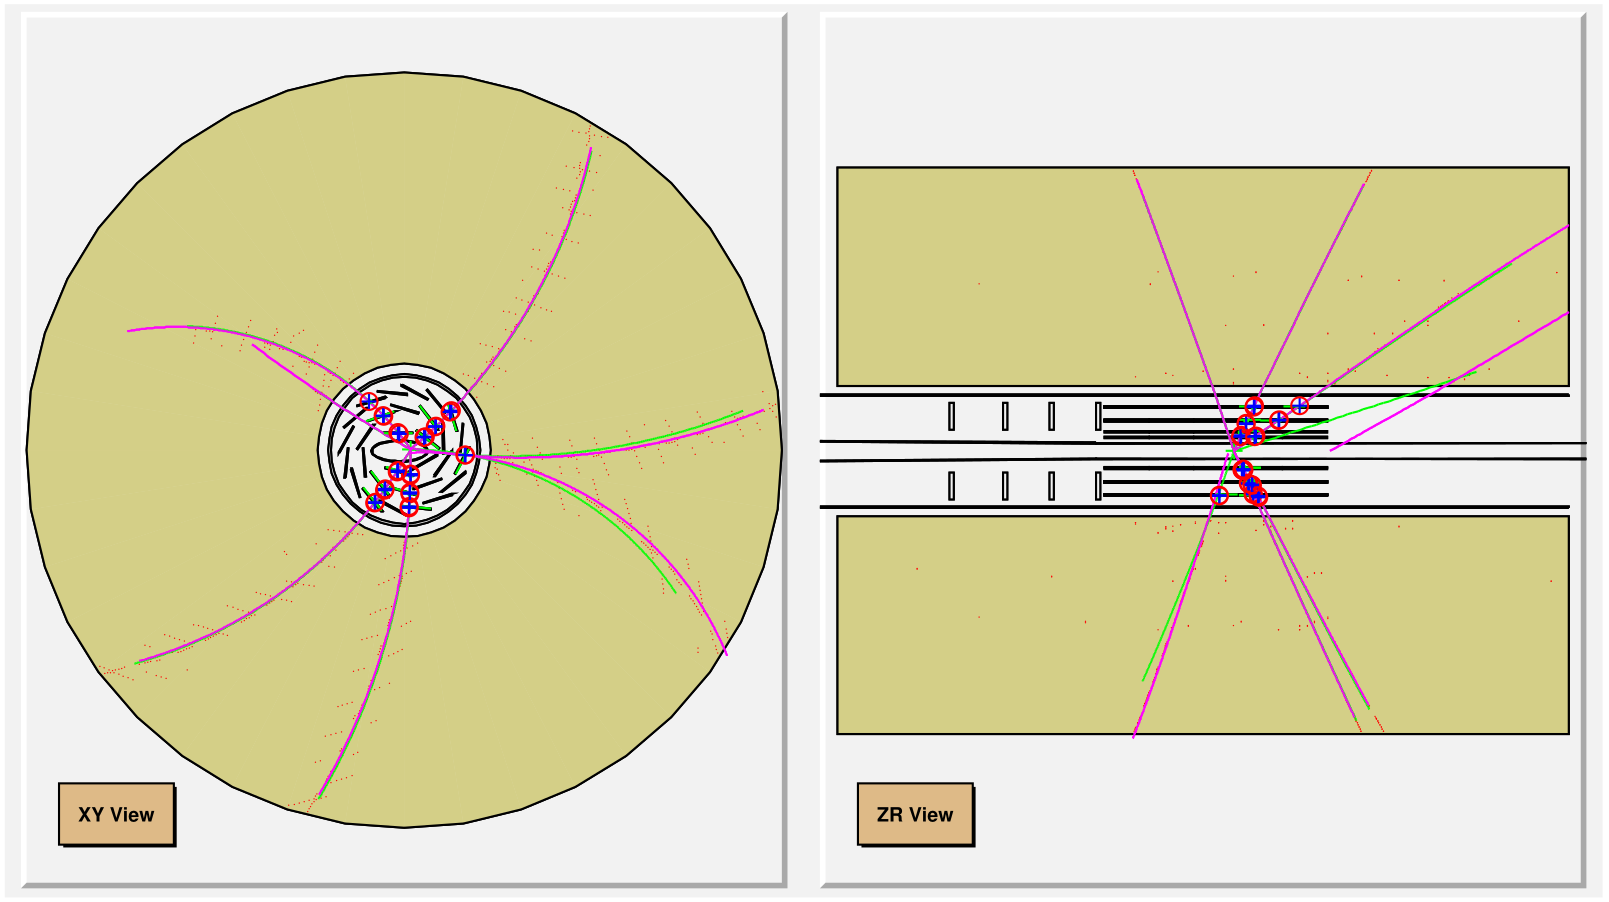
\includegraphics[width=0.80\textwidth]{pics/zeus_tracks.png}
\end{frame}

\begin{frame}
	\frametitle{Реконструкція інваріантної маси $D^{+}\to K^{-}\pi^{+}\pi^{+}$ }
	
	%{\scriptsize ZEUS Coll., H. Abramowicz et al., ``Measurement of $D^{\pm}$ production in deep inelastic $ep$ scattering with the ZEUS detector at HERA'', JHEP05 (2013) 023 \href{https://arxiv.org/abs/1302.5058}{[arXiv:1302.5058]}}
	
	\centering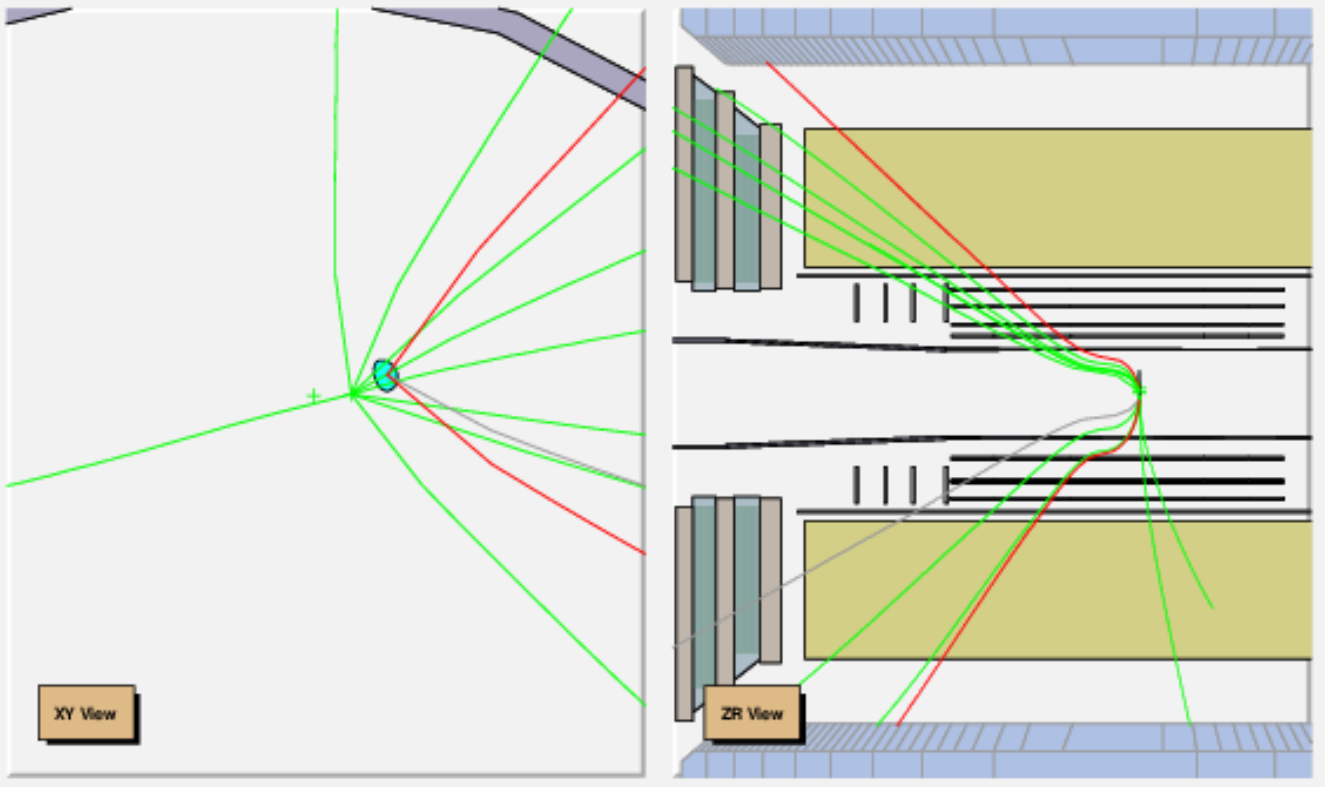
\includegraphics[width=0.85\textwidth]{pics/zeus_dplus.png}
\end{frame}

\begin{frame}
	\frametitle{Реконструкція інваріантної маси $D^{+}\to K^{-}\pi^{+}\pi^{+}$ }
	
	\centering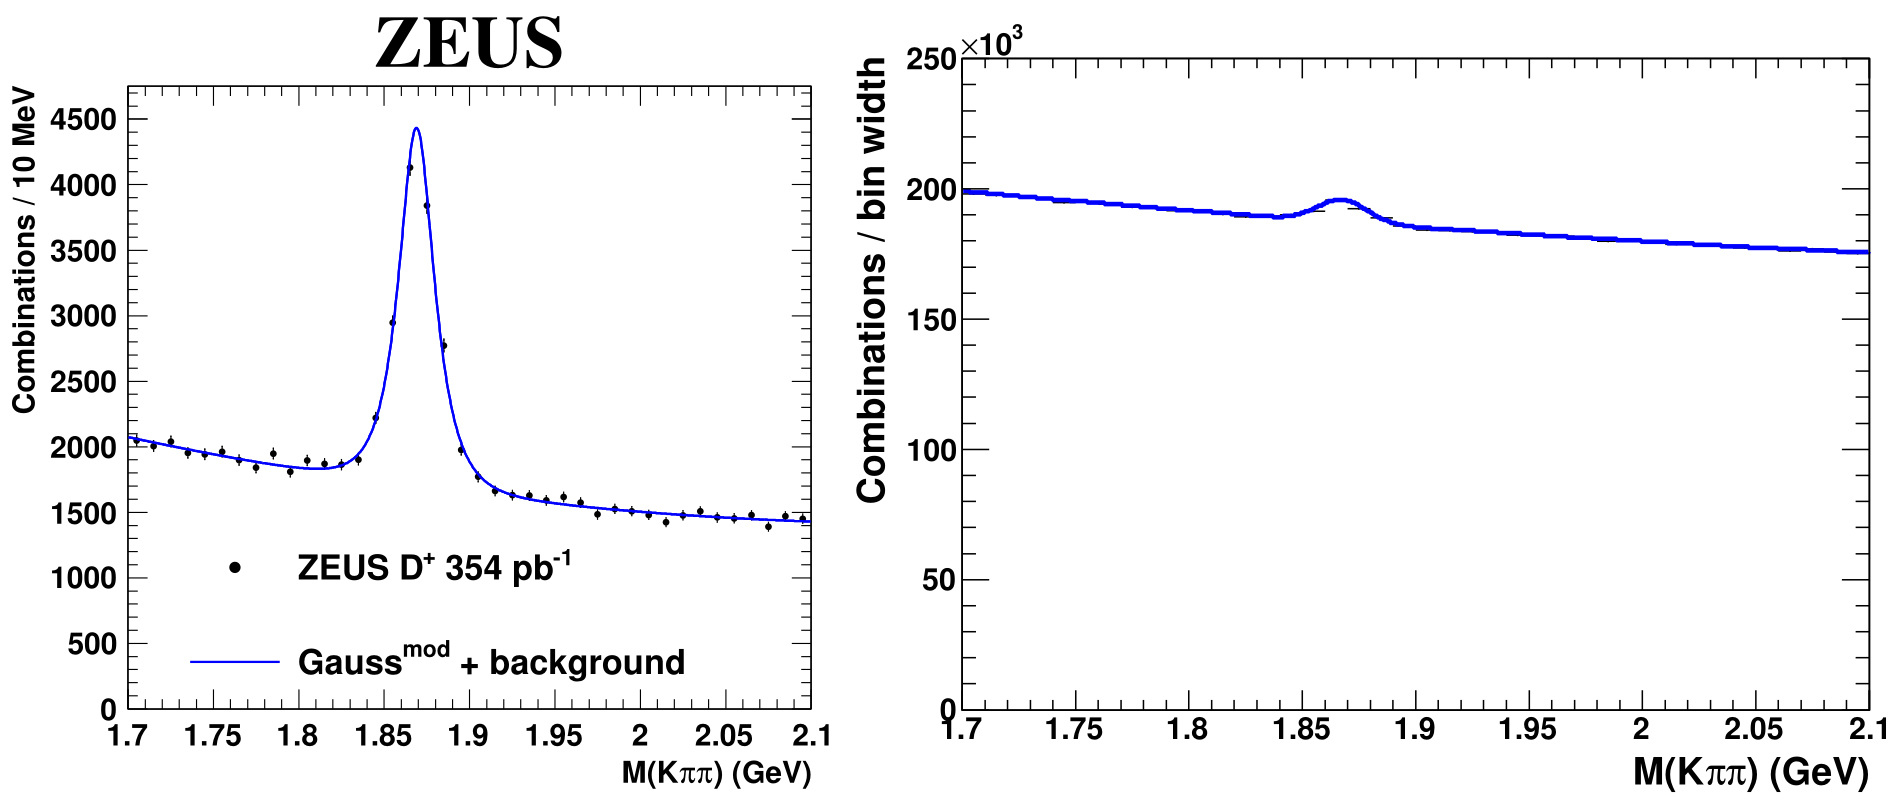
\includegraphics[width=0.85\textwidth]{pics/zeus_dplus_mass.png}
	
	\begin{itemize}
		\item $D^{+}$ складається з $c\bar{d}$ кварків
		\item $M(D^{+}) = 1869.66 \pm 0.05$ ГеВ [Particle Data Group (PDG) \url{https://pdg.lbl.gov/}]
		\item $\tau(D^{+}) = (1.033 \pm 0.005) \times 10^{-12}$ с: розпадається за рахунок слабкої взаємодії
		\item Маючи імпульс $\sim$ ГеВ, пролітає $L = \frac{p}{M} c \tau \sim$ декілька мм $\to$ його точка розпаду (вершина) може бути реконструйована $\to$ це дозволяє суттєво зменшити комбінаторний фон
	\end{itemize}
\end{frame}

\begin{frame}
	\frametitle{Практичне заняття}
	\url{https://github.com/zenaiev/hep/invmass/invmass.py}
	
	\vspace{0.05\textheight}
	\begin{itemize}
		\item Згенерувати $N$ подій
		\item У кожній події згенерувати дві частинки: $K^0$ і $D^0$ мезони
		\item Згенерувати розпади $K^0 \to \pi^{+}\pi^{-}$, $D^0 \to K^{-}\pi^{+}$
		\item Реконструювати інваріанту масу кожної пари дочірних частинок
		\item Зафітувати (fit: апроксимація, регресія) спектр інваріантної маси, визначити маси і кількість  реконструйованих частинок
		\item Намалювати графік інваріантної маси
		\item Зберегти згенеровані дані в ROOT файл і зчитати дані із нього
	\end{itemize}
\end{frame}

%\appendix
%\backupbegin
%\begin{frame}
%\frametitle{}
%\centering{\Huge \bf BACKUP}
%\end{frame}
%\backupend

\end{document}
